\section{DrawAFriend: The Game}

\begin{figure}
  \centering%
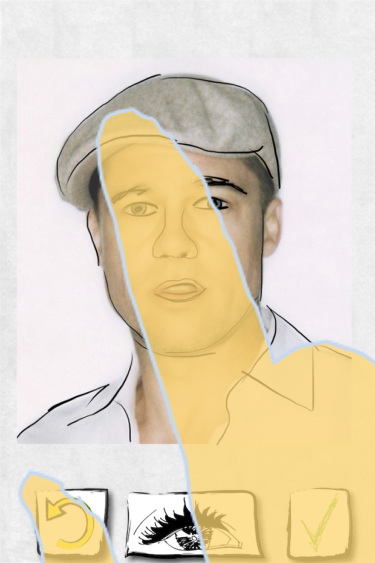
\includegraphics[width=1.5in]{DaF/PicHand2.png}
\hspace{0.1in}
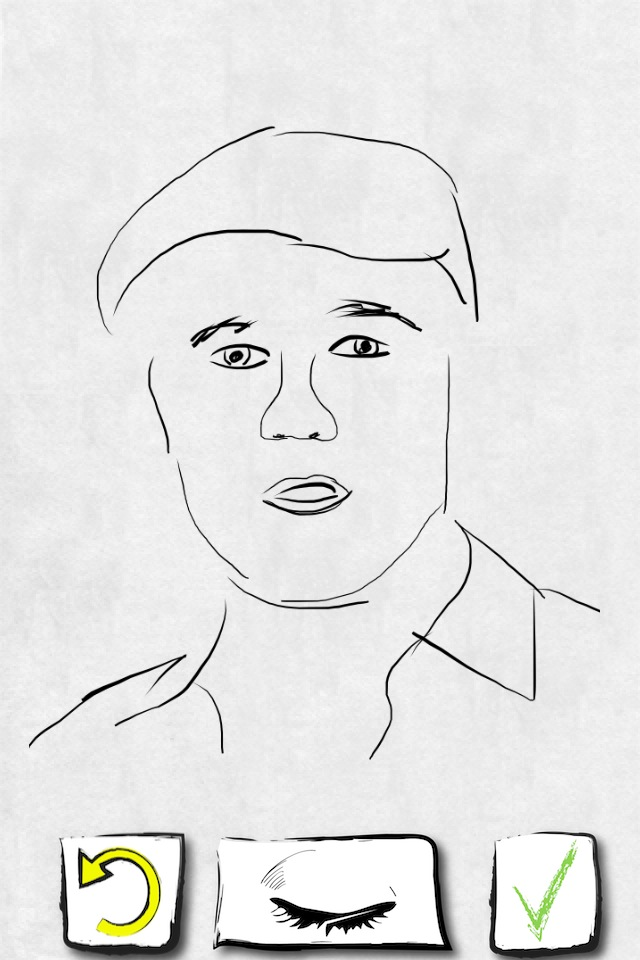
\includegraphics[width=1.5in]{DaF/IMG_3044.jpg}
  \caption{DrawAFriend: tracing a photo (left), the drawing alone (right).}
  \label{fig:DaF}
\end{figure}

\begin{figure}
  \centering%
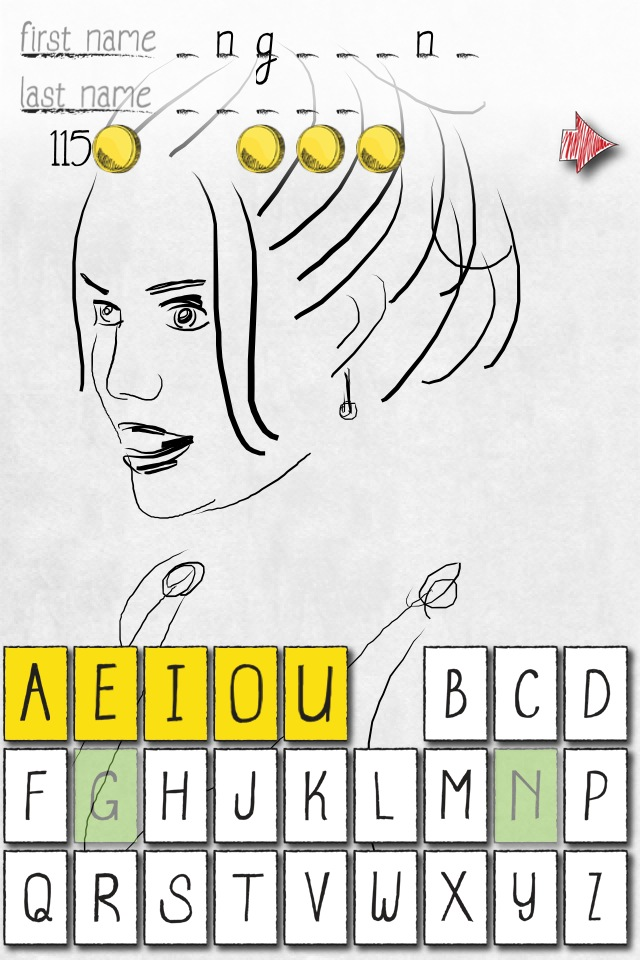
\includegraphics[width=1.5in]{DaF/IMG_3032.jpg}
\hspace{0.1in}
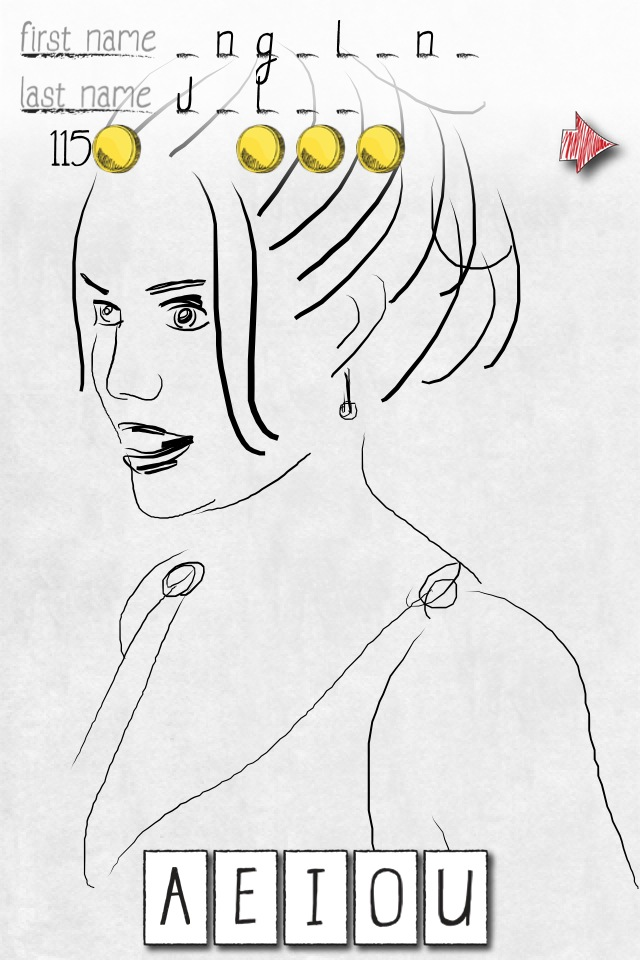
\includegraphics[width=1.5in]{DaF/IMG_3033.jpg}
  \caption{DrawAFriend: guessing identity (left), guessing final vowels (right).}
  \label{fig:DaF2}
\end{figure}

We have developed DrawAFriend, a Facebook-integrated turn-based drawing and guessing game for .  It works as follows. Players have an option to start a game with either a facebook friend or a random player on the internet. The player is then given four pictures which he can draw. These will either be mutual facebook friends' profile pictures or in the case of a random player, celebrity photos.

After choosing a photo to draw, the player is brought to the drawing screen. There he/she can trace the image (Figure~\ref{fig:DaF} left). At any point the user can press the {\em eye} button to hide the photo and see their drawing on its own (Figure~\ref{fig:DaF} right). To overcome the size limitations of the phone's size, and touch screen inaccuracies, players can zoom using the pinch zoom gesture.
Once finished, the player sends his/her drawing to the friend (or random player) whom he is playing the game with. The friend will receive a notification that they have a drawing to guess. Once the drawing is complete, the user is prompted to guess the identity of another player's drawing (Figure~\ref{fig:DaF2} left). The user sees a replay of the drawing being made, and similar to hangman, the player can guess which letters are in the mutual friend or celebrity's name. Once all the consonants are guessed the final vowels are offered to complete the guess (Figure~\ref{fig:DaF2} right).

The tracing paradigms results in a set of pre-aligned drawings. By observing the guesses we can indirectly evaluate the quality of the drawings. We hypothesize that a good drawing is much more likely to be guessed correctly than a bad drawing. DrawAFriend thus converts a dataset of quality photos , (Faceboook profile pictures) and celebrity images into a large dataset of user created drawings. This collection includes much more than the drawings themselves, but also the individually drawn strokes represented as polylines along with timing information. This dataset will include drawings from artists around the world with different artistic and cultural backgrounds.

For the purposes of the second goal of this paper, to develop an aid for helping users overcome the limitations of the mobile device while drawing, we focus on the corpus of celebrity drawings since we have a sufficient number (on average 100 per celebrity) of drawings from the same photographs by many different artists. All the drawings are not created equal. While we did not want to pass judgment on different styles, certain drawings appear to be random scribbles by people simply trying out the game. We manually removed these from our database. 

